% !TeX root = report.tex
\documentclass{ctexart}

\usepackage{xcolor}
\usepackage{subcaption}
\usepackage{hyperref}
\usepackage{mathtools}

\usepackage{tikz}
\usetikzlibrary{3d}

\title{六自由度机械臂系统建模分析}
\author{***REMOVED*** \\ ***REMOVED***}

\begin{document}

\maketitle

\section{问题简述}

随着工业自动化的大规模发展,机械臂在生产中得到了大规模的使用。
在众多机械臂中,三自由度机械臂凭借结构简单、控制容易以及造价低廉等优势受到青睐,因此也成为重要的研究对象。

本技术报告将对一个经典的三自由度机械臂以及机械臂末端安装的三自由度机械手进行运动学分析、动力学分析和控制仿真。
该机械臂总共具有六个自由度,能够在三维空间中自由运动,实现指定的目标。

\subsection{机械臂模型}

% !TeX root = ..\report.tex

\begin{figure}[ht]
    \centering
    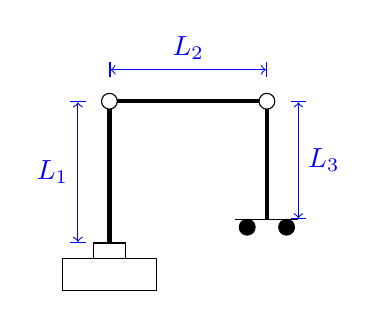
\begin{tikzpicture}
        % Arm 1 and foundation
        \draw (0.6, 0) rectangle (-0.6, -0.4);
        \draw (0.2, 0.2) rectangle (-0.2, 0);
        \draw [ultra thick] (0, 0.2) -- (0, 2);

        % Arm 2 and joint
        \draw [ultra thick] (0, 2) -- (2, 2);
        \draw [fill=white] (0, 2) circle [radius=0.1];
        
        % Arm 3 and joint
        \draw [ultra thick] (2,2) -- (2,0.5);
        \draw [fill=white] (2,2) circle [radius=0.1];
        \draw (1.6, 0.5) -- (2.4, 0.5);
        \draw [fill=black] (1.75, 0.4) circle [radius=0.1];
        \draw [fill=black] (2.25, 0.4) circle [radius=0.1];

        % Annotations
        \draw [|<->|, blue] (-0.4, 0.2) -- (-0.4, 2) node [pos=0.5, left] {$L_1$};
        \draw [|<->|, blue] (0, 2.4) -- (2, 2.4) node [pos=0.5, above] {$L_2$};
        \draw [|<->|, blue] (2.4, 2) -- (2.4, 0.5) node [pos=0.5, right] {$L_3$};
    \end{tikzpicture}
    \caption{机械臂主体部分示意图}
    \label{fig:robotic-arm-schema}
\end{figure}


本报告研究的机械臂系统由两个部分组成,第一个部分为具有三个旋转关节的三自由度机械臂,能够实现较大范围的自主运动;
第二个部分为机械臂末端安装的机械手型装置,该手型装置也具有三个自由度,能够实现对手持仪器的紧密操作。
该机械手型装置可视为一个三自由度关节,也视为三个紧邻的单自由度关节。
由于机械手的质量相对于机械臂主体可忽略,在动力学分析中可以不对后三个关节进行建模。
机械臂主体部分的示意图见图\ref{fig:robotic-arm-schema}。

\section{运动学模型}

我们使用机器人学中广泛应用的\emph{Denavit-Hartenberg 方法}为每一个关节分配固连坐标系并进行运动学分析。
按照以下约定选择和每个关节$i$与连杆$\{i\}$固连的坐标系:
\begin{enumerate}
    \item 坐标系的Z轴$\hat Z_i$与$i$号关节方向重合;
    \item 原点选择在连杆两端关节轴线的公垂线与$i$号关节的轴线交点处;
    \item X轴$\hat X_i$沿公垂线指向$i+1$号关节,若公垂线长度为零,则选择$\hat Z_i$与$\hat Z_{i+1}$构成的平面的法线;
    \item 按组成右手坐标系的原则选择Y轴$\hat Y_i$。
\end{enumerate}
分配的坐标系如图\ref{fig:affixed-frame}所示。

% !TeX root = ..\report.tex

\begin{figure}[ht]
    \centering
    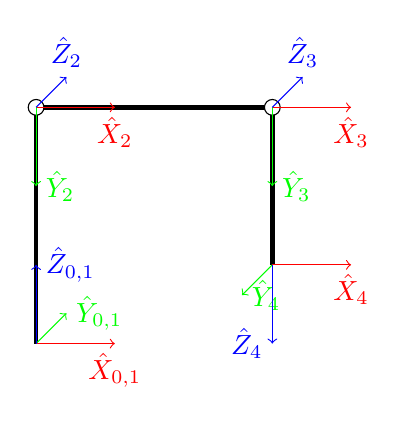
\begin{tikzpicture}
        % Arm 1
        \draw [ultra thick] (0, 0) -- (0, 3);

        \draw [->, red] (0,0,0) -- (1,0,0) node [below] {$\hat X_{0,1}$};
        \draw [->, green] (0,0,0) -- (0,0,-1) node [right] {$\hat Y_{0,1}$};
        \draw [->, blue] (0,0,0) -- (0,1,0) node [right] {$\hat Z_{0,1}$};

        % Arm 2
        \draw [ultra thick] (0, 3) -- (3, 3);
        \draw [fill=white] (0, 3) circle [radius=0.1];
        \draw [->, red] (0,3,0) -- (1,3,0) node [below] {$\hat X_2$};
        \draw [->, green] (0,3,0) -- (0,2,0) node [right] {$\hat Y_2$};
        \draw [->, blue] (0,3,0) -- (0,3,-1) node [above] {$\hat Z_2$};

        % Arm 3 and joint
        \draw [ultra thick] (3,3) -- (3,1);
        \draw [fill=white] (3,3) circle [radius=0.1];
        \draw [->, red] (3,3,0) -- (4,3,0) node [below] {$\hat X_3$};
        \draw [->, green] (3,3,0) -- (3,2,0) node [right] {$\hat Y_3$};
        \draw [->, blue] (3,3,0) -- (3,3,-1) node [above] {$\hat Z_3$};
        
        % Frame 4
        \draw [->, red] (3,1,0) -- (4,1,0) node [below] {$\hat X_4$};
        \draw [->, green] (3,1,0) -- (3,1,1) node[right] {$\hat Y_4$};
        \draw [->, blue] (3,1,0) -- (3,0,0) node[left] {$\hat Z_4$};
    \end{tikzpicture}
    \caption{固连坐标系分配}
    \label{fig:affixed-frame}
\end{figure}


按照指定的方法分配每个关节的固连坐标系后,可得出每个关节的 Denavit-Hartenberg 参数。
\begin{enumerate}
    \item $\alpha_i$是轴$\hat Z_i$与$\hat Z_{i+1}$绕$\hat X_i$方向的夹角;
    \item $a_i$是轴$\hat Z_i$与$\hat Z_{i+1}$沿$\hat X_i$方向的距离;
    \item $d_i$是轴$\hat X_{i-1}$与$\hat X_i$沿$\hat Z_i$方向的距离;
    \item $\theta_i$是轴$\hat X_{i-1}$与$\hat X_i$绕$\hat Z_i$方向的夹角。
\end{enumerate}
计算的参数如表\ref{tab:DH-params}所示。

\begin{table}[ht]
    \caption{Denavit-Hartenberg参数}
    \label{tab:DH-params}
    \centering
    \begin{tabular}{c|cccc}
        \hline
        & $\alpha_{i-1}$ & $a_{i-1}$ & $d_i$ & $\theta_i$ \\
        \hline
        1 & $0$ & $0$ & $0$ & $\theta_1$ \\
        2 & $-\frac{\pi}{2}$ & $L_1$ & $0$ & $\theta_2$ \\
        3 & $0$ & $L_2$ & $0$ & $\theta_3$ \\
        4 & $-\frac{\pi}{2}$ & $L_3$ & $0$ & $\theta_4$\\
        5 & $\frac{\pi}{2}$ & $0$ & $0$ & $\theta_5$\\
        6 & $-\frac{\pi}{2}$ & $0$ & $0$ & $\theta_6$\\ \hline
    \end{tabular}
\end{table}

\subsection{正向运动学}

利用 Denavit-Hartenberg 参数,相邻两个坐标系之间的变换矩阵可以非常容易地表示出来,按照约定,有
\[ 
    \begin{aligned}
        \prescript{i-1}{i}{T} 
        &= R_X (\alpha_{i-1}) D_X (a_{i-1}) R_Z (\theta_i) D_Z (d_i) \\
        &= \begin{bmatrix}
            \cos \theta_i & - \sin \theta_i & 0 & \alpha_{i-1} \\
            \sin \theta_i \cos \alpha_{i-1} & \cos \theta_i \cos \alpha_{i-1} & - \sin \alpha_{i-1} & - \sin \alpha_{i-1} d_i \\
            \sin \theta_i \sin \alpha_{i-1} & \cos \theta_i \sin \alpha_{i-1} & \cos \alpha_{i-1} & \cos \alpha_{i-1} d_i \\
            0 & 0 & 0 & 1
        \end{bmatrix}
    \end{aligned}
\]

从而我们可以计算所有相邻坐标系的变换矩阵
\[
    \prescript{0}{1}{T} =
    \begin{bmatrix}
        \cos \theta_1 & - \sin \theta_1 & 0 & 0 \\
        \sin \theta_1 & \cos \theta_1 & 0 & 0 \\
        0 & 0 & 1 & 0 \\
        0 & 0 & 0 & 1
    \end{bmatrix}
\]

\[
    \prescript{1}{2}{T} =
    \begin{bmatrix}
        \cos \theta_2 & - \sin \theta_2 & 0 & L_1 \\
        0 & 0 & 1 & 0 \\
        -\sin \theta_2 & - \cos \theta_2 & 0 & 0 \\
        0 & 0 & 0 & 1
    \end{bmatrix}
\]

\[
    \prescript{2}{3}{T} = 
    \begin{bmatrix}
        \cos \theta_3 & - \sin \theta_3 & 0 & L_2 \\
        \sin \theta_3 & \cos \theta_3 & 0 & 0 \\
        0 & 0 & 1 & 0 \\
        0 & 0 & 0 & 1
    \end{bmatrix}
\]

\[
    \prescript{3}{4}{T} =
    \begin{bmatrix}
        \cos \theta_4 & - \sin \theta_4 & 0 & L_3 \\
        0 & 0 & 1 & 0 \\
        -\sin \theta_4 & - \cos \theta_4 & 0 & 0 \\
        0 & 0 & 0 & 1
    \end{bmatrix}
\]

\[
    \prescript{4}{5}{T} =
    \begin{bmatrix}
        \cos \theta_5 & - \sin \theta_5 & 0 & 0 \\
        0 & 0 & -1 & 0 \\
        \sin \theta_5 & \cos \theta_5 & 0 & 0 \\
        0 & 0 & 0 & 1
    \end{bmatrix}
\]

\[
    \prescript{5}{6}{T} =
    \begin{bmatrix}
        \cos \theta_6 & - \sin \theta_6 & 0 & 0 \\
        0 & 0 & 1 & 0 \\
        -\sin \theta_6 & - \cos \theta_6 & 0 & 0 \\
        0 & 0 & 0 & 1
    \end{bmatrix}
\]

然后我们可以利用矩阵乘法计算任何两个关节坐标系之间的变换。
首先考虑机械手外部的变换,即从坐标系$1$到坐标系$3$的变换:
\[
    \prescript{1}{3}{T} = \prescript{1}{2}{T} \prescript{2}{3}{T} =
    \begin{bmatrix}
        \cos{\left( {{\theta }_3}+{{\theta }_2}\right) } & -\sin{\left( {{\theta }_3}+{{\theta }_2}\right) } & 0 & {L_2} \cos{ {{\theta }_2} }+{L_1}\\
        0 & 0 & 1 & 0\\
        -\sin{\left( {{\theta }_3}+{{\theta }_2}\right) } & -\cos{\left( {{\theta }_3}+{{\theta }_2}\right) } & 0 & - {L_2} \sin{ {{\theta }_2} } \\
        0 & 0 & 0 & 1
    \end{bmatrix}
\]
从而
\[
    \prescript{0}{3}{T} =
    \begin{bmatrix}
        \cos \theta_1 \cos{\left( {{\theta }_3}+{{\theta }_2}\right) } & - \cos \theta_1 \sin{\left( {{\theta }_3}+{{\theta }_2}\right) }  & -\sin \theta_1 & \cos \theta_1 \left( {L_2} \cos\theta_2+{L_1}\right) \\
            \sin \theta_1 \cos{\left( {{\theta }_3}+{{\theta }_2}\right) } & - \sin \theta_1 \sin{\left( {{\theta }_3}+{{\theta }_2}\right) }  & \cos \theta_1 & \sin \theta_1 \left( {L_2} \cos\theta_2+{L_1}\right) \\
            -\sin{\left( {{\theta }_3}+{{\theta }_2}\right) } & -\cos{\left( {{\theta }_3}+{{\theta }_2}\right) } & 0 & - {L_2} \sin \theta_2 \\
            0 & 0 & 0 & 1
    \end{bmatrix}
\]

然后考虑机械手内部的变换,即从坐标系$4$到坐标系$6$的变换:
\[
    \prescript{4}{6}{T} = \prescript{4}{5}{T} \prescript{5}{6}{T} =
    \begin{bmatrix}\cos{ {{\theta }_5} } \cos{ {{\theta }_6} } & - \cos{ {{\theta }_5} } \sin{ {{\theta }_6} }  & -\sin{ {{\theta }_5} } & 0\\
        \sin{ {{\theta }_6} } & \cos{ {{\theta }_6} } & 0 & 0\\
        \sin{ {{\theta }_5} } \cos{ {{\theta }_6} } & - \sin{ {{\theta }_5} } \sin{ {{\theta }_6} }  & \cos{ {{\theta }_5} } & 0\\
        0 & 0 & 0 & 1
    \end{bmatrix}
\]
从而可得
\[
        \prescript{3}{6}{T} = \\
    \begin{bmatrix}\cos{{{\theta }_4} } \cos{ {{\theta }_5} } \cos{ {{\theta }_6} }-\sin{ {{\theta }_4} } \sin{ {{\theta }_6} } & - \cos{ {{\theta }_4} } \cos{ {{\theta }_5} } \sin{ {{\theta }_6} } -\sin{ {{\theta }_4} } \cos{ {{\theta }_6} } & - \cos{ {{\theta }_4} } \sin{ {{\theta }_5} }  & {L_3}\\
        \sin{ {{\theta }_5} } \cos{ {{\theta }_6} } & - \sin{ {{\theta }_5} } \sin{ {{\theta }_6} }  & \cos{ {{\theta }_5} } & 0\\
        - \cos{{{\theta }_4}} \sin{ {{\theta }_6} } -\sin{ {{\theta }_4} } \cos{ {{\theta }_5} } \cos{ {{\theta }_6} } & \sin{ {{\theta }_4} } \cos{ {{\theta }_5} } \sin{ {{\theta }_6} }-\cos{ {{\theta }_4} } \cos{ {{\theta }_6} } & \sin{ {{\theta }_4} } \sin{ {{\theta }_5} } & 0\\
        0 & 0 & 0 & 1
    \end{bmatrix}
\]

将所有矩阵依次相乘,即可得到本机械臂系统的运动学方程。
\[
    \prescript{0}{6}{T} = \begin{bmatrix}
        r_{11} & r_{12} & r_{13} & p_x \\
        r_{21} & r_{22} & r_{23} & p_y \\
        r_{31} & r_{32} & r_{33} & p_z \\
        0 & 0 & 0 & 1
    \end{bmatrix}
\]
其中
\[
    \begin{aligned}
        r_{11} = & \cos\theta_1 \left( \cos{\left( {{\theta }_3}+{{\theta }_2}\right) } \left( \cos\theta_4 \cos\theta_5 \cos\theta_6-\sin\theta_4 \sin\theta_6\right) - \sin{\left( {{\theta }_3}+{{\theta }_2}\right) } \sin\theta_5 \cos\theta_6\right) \\ 
        &-\sin\theta_1 \left( -\left( \cos\theta_4 \sin\theta_6\right) -\sin\theta_4 \cos\theta_5 \cos\theta_6\right)   \\
        r_{12} = & \cos\theta_1 \left( \cos{\left( {{\theta }_3}+{{\theta }_2}\right) } \left( -\left( \cos\theta_4 \cos\theta_5 \sin\theta_6\right) -\sin\theta_4 \cos\theta_6\right) +\sin{\left( {{\theta }_3}+{{\theta }_2}\right) } \sin\theta_5 \sin\theta_6\right) \\ 
        &-\sin\theta_1 \left( \sin\theta_4 \cos\theta_5 \sin\theta_6-\cos\theta_4 \cos\theta_6\right) \\
        r_{13} = & \cos\theta_1 \left( -\left( \cos{\left( {{\theta }_3}+{{\theta }_2}\right) } \cos\theta_4 \sin\theta_5\right) -\sin{\left( {{\theta }_3}+{{\theta }_2}\right) } \cos\theta_5\right) -\sin\theta_1 \sin\theta_4 \sin\theta_5 \\
        r_{21} = & \sin\theta_1 \left( \cos{\left( {{\theta }_3}+{{\theta }_2}\right) } \left( \cos\theta_4 \cos\theta_5 \cos\theta_6-\sin\theta_4 \sin\theta_6\right) -\sin{\left( {{\theta }_3}+{{\theta }_2}\right) } \sin\theta_5 \cos\theta_6\right) \\
        &+\cos\theta_1 \left( -\left( \cos\theta_4 \sin\theta_6\right) -\sin\theta_4 \cos\theta_5 \cos\theta_6\right) \\
        r_{22} = & \sin\theta_1 \left( \cos{\left( {{\theta }_3}+{{\theta }_2}\right) } \left( -\left( \cos\theta_4 \cos\theta_5 \sin\theta_6\right) -\sin\theta_4 \cos\theta_6\right) +\sin{\left( {{\theta }_3}+{{\theta }_2}\right) } \sin\theta_5 \sin\theta_6\right) \\
        & +\cos\theta_1 \left( \sin\theta_4 \cos\theta_5 \sin\theta_6-\cos\theta_4 \cos\theta_6\right) \\
        r_{23} = & \sin\theta_1 \left( -\left( \cos{\left( {{\theta }_3}+{{\theta }_2}\right) } \cos\theta_4 \sin\theta_5\right) -\sin{\left( {{\theta }_3}+{{\theta }_2}\right) } \cos\theta_5\right) +\cos\theta_1 \sin\theta_4 \sin\theta_5 \\
        r_{31} = &  -\left( \sin{\left( {{\theta }_3}+{{\theta }_2}\right) } \left( \cos\theta_4 \cos\theta_5 \cos\theta_6-\sin\theta_4 \sin\theta_6\right) \right) -\cos{\left( {{\theta }_3}+{{\theta }_2}\right) } \sin\theta_5 \cos\theta_6 \\
        r_{32} = & \cos{\left( {{\theta }_3}+{{\theta }_2}\right) } \sin\theta_5 \sin\theta_6-\sin{\left( {{\theta }_3}+{{\theta }_2}\right) } \left( -\left( \cos\theta_4 \cos\theta_5 \sin\theta_6\right) -\sin\theta_4 \cos\theta_6\right) \\
        r_{33} = & \sin{\left( {{\theta }_3}+{{\theta }_2}\right) } \cos\theta_4 \sin\theta_5-\cos{\left( {{\theta }_3}+{{\theta }_2}\right) } \cos\theta_5 \\
        p_x = & \cos{\theta_1} \left( {L_3} \cos{\left( {{\theta }_3}+{{\theta }_2}\right) }+{L_2} \cos{\theta_2}+{L_1}\right) \\
        p_y = & \sin{\theta_1} \left( {L_3} \cos{\left( {{\theta }_3}+{{\theta }_2}\right) }+{L_2} \cos{\theta_2}+{L_1}\right)  \\
        p_z = & -{L_3} \sin{\left( {{\theta }_3}+{{\theta }_2}\right) } -{L_2} \sin{\theta_2}
    \end{aligned}
\]
这就完成了对该机械臂系统的运动学分析。

\subsection{逆向运动学}

根据我们已完成的运动学分析,通过求解方程即可得到逆运动学关系。
注意到仿射变换$\prescript{0}{6}{T}$的平移部分$p_x, p_y, p_z$仅仅与前三个关节的夹角有关,我们可以先求解这三个夹角,即$\theta_1, \theta_2$和$\theta_3$。
列出以下方程:
\begin{eqnarray}
    \label{eqn:ik-1}
    p_x & = & \cos{\theta_1} \left( {L_3} \cos{\left( {{\theta }_3}+{{\theta }_2}\right) }+{L_2} \cos{\theta_2}+{L_1}\right) \\
    \label{eqn:ik-2}
    p_y & = & \sin{\theta_1} \left( {L_3} \cos{\left( {{\theta }_3}+{{\theta }_2}\right) }+{L_2} \cos{\theta_2}+{L_1}\right)  \\
    \label{eqn:ik-3}
    p_z & = & -{L_3} \sin{\left( {{\theta }_3}+{{\theta }_2}\right) } -{L_2} \sin{\theta_2}
\end{eqnarray}
将方程\eqref{eqn:ik-1}与\eqref{eqn:ik-2}相除,即可得到
\begin{equation}
    \label{eqn:ik-theta-one}
    \frac{\sin \theta_1}{\cos \theta_1} = \tan \theta_1 = \frac{p_y}{p_x}
\end{equation}
将方程\eqref{eqn:ik-1}移项并平方,可得
\begin{equation*}
    \left( \frac{p_x}{\cos \theta_1} - L_1 \right)^2 =
    L_3^2 \cos^2(\theta_3 + \theta_2) + L_2^2 \cos^2 (\theta_2) + 2 L_3 L_2 \cos (\theta_3 + \theta_2) \cos (\theta_2)
\end{equation*}
将\eqref{eqn:ik-3}平方并与上式相加,得到
\begin{eqnarray}
    \label{eqn:ik-theta-three}
    \left( \frac{p_x}{\cos \theta_1} - L_1 \right)^2 + p_z^2 
    & = & L_3^2 + L_2^2 + 2 L_3 L_2 \left( \cos(\theta_3 + \theta_2) \cos \theta_2 + \sin(\theta_3 + \theta_2) \sin \theta_2 \right) \nonumber \\
    & = & L_3^2 + L_2^2 + 2 L_3 L_2 \cos \theta_3 \nonumber \\
    \implies \cos \theta_3 & = & \frac{\left( \frac{p_x}{\cos \theta_1} - L_1 \right)^2 + p_z^2 - L_2^2 - L_3^2}{2 L_2 L_3}
\end{eqnarray}
最后,将方程\eqref{eqn:ik-3}利用和角公式展开,得到
\begin{equation*}
    - p_z = L_3 (\sin \theta_2 \cos \theta_3 + \cos \theta_2 \sin \theta_3) + L_2 \sin \theta_2
\end{equation*}
利用$u = \tan \frac{\theta_2}{2}$转化为多项式进行求解,得到
\begin{eqnarray*}
    - p_z (1 + u^2) &=& L_3 (2u \cos \theta_3 + (1 - u^2) \sin \theta_3) + 2 L_2 u \\
    0 &=& (p_z - L_3 \sin \theta_3) u^2 + (2 L_2 + 2 L_3 \cos \theta_3) u + L_3 \sin \theta_3 + p_z
\end{eqnarray*}
求解该二次方程即可得到$\theta_2$,这就完成了机械臂部分逆向运动学的求解。

接下来考虑求解机械手的逆向运动学模型,即求解$\theta_4$、$\theta_5$和$\theta_6$。
我们已经通过计算求得了$\theta_1$、$\theta_2$和$\theta_3$,因此变换$\prescript{0}{1}{T}$、$\prescript{1}{2}{T}$和$\prescript{2}{3}{T}$可视为是已知的。
考虑将方程进行分离变量:
\[ 
    \prescript{0}{6}{T} = \prescript{0}{3}{T}(\theta_1, \theta_2, \theta_3) \cdot \prescript{3}{6}{T} (\theta_4, \theta_5, \theta_6)
    \iff
    \prescript{0}{3}{T^{-1}} (\theta_1, \theta_2, \theta_3) \cdot \prescript{0}{6}{T} = \prescript{3}{6}{T} (\theta_4, \theta_5, \theta_6)
\]
注意到在变换矩阵$\prescript{3}{6}{T}$中,有几个组成非常简单的元素
\[
    \prescript{3}{6}{T} = \\
    \begin{bmatrix}
        c{{{\theta }_4} } c{ {{\theta }_5} } c{ {{\theta }_6} }-s{ {{\theta }_4} } s{ {{\theta }_6} } & 
        - c{ {{\theta }_4} } c{ {{\theta }_5} } s{ {{\theta }_6} } -s{ {{\theta }_4} } c{ {{\theta }_6} } & 
        \textcolor{red}{- \cos\theta_4 \sin\theta_5 } &
        {L_3}\\
        \textcolor{green}{\sin{ {{\theta }_5} } \cos{ {{\theta }_6} }} & 
        \textcolor{green}{- \sin{ {{\theta }_5} } \sin{ {{\theta }_6} }}  & 
        \textcolor{blue}{\cos{ {{\theta }_5} }}
        & 0\\
        - c{{{\theta }_4}} s{ {{\theta }_6} } -s{ {{\theta }_4} } c{ {{\theta }_5} } c{ {{\theta }_6} } &
        s{ {{\theta }_4} } c{ {{\theta }_5} } s{ {{\theta }_6} }-c{ {{\theta }_4} } c{ {{\theta }_6} } &
        \textcolor{red}{ \sin\theta_4 \sin\theta_5} & 0\\
        0 & 0 & 0 & 1
    \end{bmatrix}
\]
我们可将矩阵等式两侧的红色、蓝色和绿色项分别相等,从而得到五个方程。
将红色项两个方程相除,即可得到$\tan \theta_4$,从而解出$\theta_4$。
从蓝色项即可得到$\cos \theta_5$,从而解出$\theta_5$。
将绿色项两个方程相除,即可得到$- \tan \theta_6$,从而解出$\theta_6$。

这就完成了对机械手的逆向运动学分析。

\section{动力学模型}

接下来我们将研究该机械臂主体部分的动力学模型。
我们首先计算每个关节与连杆的速度和角速度,然后利用拉格朗日方程给出该系统的动力学方程。

\subsection{计算速度和角速度}

关节处的速度和关节之间连杆的角速度可以用以下方程迭代地求出
\begin{eqnarray*}
    \prescript{i+1}{}{\omega_{i+1}} 
    &=& \prescript{i+1}{i}{R} \prescript{i}{}{\omega_i} + \dot \theta_{i+1} \prescript{i+1}{}{\hat Z_{i+1}} 
    = \prescript{i+1}{i}{R} \prescript{i}{}{\omega_i} + \begin{bmatrix}
        0 \\ 0 \\ \dot \theta_{i+1}
    \end{bmatrix}\\
    \prescript{i+1}{}{v_{i+1}} 
    &=& \prescript{i+1}{i}{R} (\prescript{i}{}{v_i} + \prescript{i}{ }{\omega_i} \times \prescript{i}{}{P_{i+1}})
\end{eqnarray*}
其中$\prescript{i}{}{P_{i+1}}$表示从坐标系$i$的原点到$i+1$的原点的向量在坐标系$i$中的坐标。

我们只考虑机械臂的主体部分,从而只需要以下四个矩阵:
\begin{eqnarray*}
    \prescript{0}{1}{R} &=&
    \begin{bmatrix}
        \cos \theta_1 & - \sin \theta_1 & 0  \\
        \sin \theta_1 & \cos \theta_1 & 0  \\
        0 & 0 & 1  \\
    \end{bmatrix} \\
    \prescript{1}{2}{R} &=&
    \begin{bmatrix}
        \cos \theta_2 & - \sin \theta_2 & 0  \\
        0 & 0 & 1 \\
        -\sin \theta_2 & - \cos \theta_2 & 0
    \end{bmatrix} \\
    \prescript{2}{3}{R} &=&
    \begin{bmatrix}
        \cos \theta_3 & - \sin \theta_3 & 0  \\
        \sin \theta_3 & \cos \theta_3 & 0 \\
        0 & 0 & 1
    \end{bmatrix} \\
    \prescript{3}{4}{R} &=&
    \begin{bmatrix}
        \cos \theta_4 & - \sin \theta_4 & 0 \\
        0 & 0 & 1 \\
        -\sin \theta_4 & - \cos \theta_4 & 0
    \end{bmatrix} \\
\end{eqnarray*}

我们依次考虑每个关节。
对关节一,有
\[
    \prescript{1}{}{\omega_1} = \begin{bmatrix}
        0 \\ 0 \\ \dot \theta_1
    \end{bmatrix}, \quad
    \prescript{1}{}{v_1} = \vec 0
\]
对关节二,有
\[
    \begin{aligned}
    \prescript{2}{}{\omega_2} = & 
    \begin{bmatrix}
        \cos \theta_2 & - \sin \theta_2 & 0  \\
        0 & 0 & 1 \\
        -\sin \theta_2 & - \cos \theta_2 & 0
    \end{bmatrix}^\top 
    \begin{bmatrix}
        0 \\ 0 \\ \dot \theta_1
    \end{bmatrix} +
    \begin{bmatrix}
        0 \\ 0 \\ \dot \theta_2
    \end{bmatrix} \\
    = & \begin{bmatrix}
        -\dot \theta_1 \sin\theta_2 \\
        -\dot \theta_1 \cos\theta_2 \\
        \dot \theta_2
    \end{bmatrix} \\
    \prescript{2}{}{v_2} = &
    \begin{bmatrix}
        \cos \theta_2 & - \sin \theta_2 & 0  \\
        0 & 0 & 1 \\
        -\sin \theta_2 & - \cos \theta_2 & 0
    \end{bmatrix}^\top 
    \left(
        \begin{bmatrix}
            0 \\ 0 \\ \dot \theta_1
        \end{bmatrix}
        \times
        \begin{bmatrix}
           L_1 \\ 0 \\ 0 
        \end{bmatrix}
    \right) \\ = & \begin{bmatrix}
        0 \\ 0 \\ L_1 \dot\theta_1
    \end{bmatrix}
    \end{aligned}
\]
对关节三,有
\[
    \begin{aligned}
        \prescript{3}{}{\omega_3} = &
        \begin{bmatrix}
            \cos \theta_3 & - \sin \theta_3 & 0  \\
            \sin \theta_3 & \cos \theta_3 & 0 \\
            0 & 0 & 1
        \end{bmatrix}^\top
        \begin{bmatrix}
            - \dot \theta_1 \sin \theta_2 \\
            - \dot \theta_1 \cos \theta_2 \\
            \dot \theta_2
        \end{bmatrix}
        +
        \begin{bmatrix}
            0 \\ 0 \\ \dot \theta_3
        \end{bmatrix} \\
        = &
        \begin{bmatrix}
            -\dot\theta_1 \cos\theta_2 \sin\theta_3 -\dot\theta_1 \sin\theta_2 \cos\theta_3\\
            \dot\theta_1 \sin\theta_2 \sin\theta_3 - \dot\theta_1 \cos\theta_2 \cos\theta_3\\
            \dot\theta_3 + \dot\theta_2
        \end{bmatrix}
        \\
        \prescript{3}{}{v_3} = & 
        \begin{bmatrix}
            \cos \theta_3 & - \sin \theta_3 & 0  \\
            \sin \theta_3 & \cos \theta_3 & 0 \\
            0 & 0 & 1
        \end{bmatrix}^\top
        \left( \begin{bmatrix}
            0 \\ 0 \\ L_1 \dot\theta_1
            \end{bmatrix} +
            \begin{bmatrix}
            -\dot \theta_1 \sin\theta_2 \\
            -\dot \theta_1 \cos\theta_2 \\
            \dot \theta_2
        \end{bmatrix}
        \times \begin{bmatrix}
            L_2 \\ 0 \\ 0
        \end{bmatrix} \right) \\
        = &
        \begin{bmatrix}
            \cos \theta_3 & - \sin \theta_3 & 0  \\
            \sin \theta_3 & \cos \theta_3 & 0 \\
            0 & 0 & 1
        \end{bmatrix}^\top
        \begin{bmatrix}
            0 \\ L_2 \dot \theta_2 \\ L_2 \dot \theta_1 \cos \theta_2 + L_1 \dot\theta_1
        \end{bmatrix} \\
        = & \begin{bmatrix}
            {L_2} \dot\theta_2 \sin\theta_3\\
                {L_2} \dot\theta_2 \cos\theta_3\\
                {L_2} \dot\theta_1 \cos\theta_2 + L_1 \dot\theta_1
        \end{bmatrix}
    \end{aligned}
\]

\subsection{拉格朗日方程}

为了使用拉格朗日方程进行动力学求解,我们需要知道每个连杆质心的速度和连杆的角速度。
连杆刚体的角速度已经在上一节中求出了,因此我们只需要知道各连杆的质心速度。
我们知道拉格朗日量的定义为
\[ \mathcal L = \mathcal T - \mathcal V = \frac{1}{2} m v_c^\top v_c + \frac{1}{2} \prescript{i}{}{\omega_i}^\top \mathbf I \prescript{i}{}{\omega_i} - \mathcal V\]
其中的平动动能与坐标系的选择无关,因此我们可以任取坐标系求解质心速度。

\subsubsection{计算动能}

假设连杆的质量均匀分布,则
\[
\prescript{i}{}{v_{c_{i}}} 
    = \prescript{i}{}{v_i} + \prescript{i}{ }{\omega_i} \times \frac{1}{2} \prescript{i}{}{P_{i+1}}
\]
我们依次计算连杆的质心速度,对连杆一,
\[
    \prescript{1}{}{v_{c_1}} = \begin{bmatrix}
        0 \\ 0 \\ \dot\theta_1
    \end{bmatrix} \times \begin{bmatrix}
        \frac{L_1}{2} \\ 0 \\ 0
    \end{bmatrix} = \begin{bmatrix}
       0 \\ \frac{L_1}{2} \dot \theta_1 \\ 0
    \end{bmatrix}
\]
考虑到其惯性张量是对称的,其动能为
\[
    \begin{aligned}
        \mathcal T_1 
        = & \frac{1}{8} m_1 L_1^2 \dot\theta_1^2 + \frac{1}{2} (I_{xx,1} \omega_x^2 + I_{yy,1} \omega_y^2 + I_{zz,1} \omega_z^2) \\
        = & \frac{1}{8} m_1 L_1^2 \dot\theta_1^2 + \frac{I_{zz,1}}{2} {\dot \theta_1}^2
    \end{aligned}
\]

对连杆二,
\[
    \begin{aligned}
        \prescript{2}{}{v_{c_2}} = &
        \begin{bmatrix}
            0 \\ 0 \\ L_1 \dot \theta_1
        \end{bmatrix} +
        \begin{bmatrix}
            -\dot \theta_1 \sin\theta_2 \\
            -\dot \theta_1 \cos\theta_2 \\
            \dot \theta_2
        \end{bmatrix} \times \begin{bmatrix}
            \frac{L_2}{2} \\ 0 \\ 0
        \end{bmatrix} \\
        = & \begin{bmatrix}
            0 \\ 
            \frac{1}{2} L_2 \dot \theta_2 \\ 
            L_1 \dot \theta_1 + \frac{1}{2} L_2 \dot \theta_1 \cos \theta_2
        \end{bmatrix}
    \end{aligned}
\]
从而其动能为
\[
    \begin{aligned}
        \mathcal T_2 = & \frac{1}{2} m_2 (\frac{L_2^2}{4} \dot \theta_2^2 + \frac{L_2^2}{4}\dot\theta_1^2 \cos^2 \theta_2 + L_1^2 \dot\theta_1^2 + L_1 L_2 \dot\theta_1^2 \cos\theta_2) \\
        & + \frac{I_{xx,2}}{2} {\dot\theta_1}^2 \sin^2\theta_2+ \frac{I_{yy,2}}{2} {\dot\theta_1}^2 \cos^2\theta_2 + \frac{I_{zz,2}}{2} {\dot\theta_2}^2\\
    \end{aligned}
\]

对连杆三,
\[
    \begin{aligned}
        \prescript{3}{}{v_{c_3}} & = \begin{bmatrix}
            {L_2} \dot\theta_2 \sin\theta_3\\
                {L_2} \dot\theta_2 \cos\theta_3\\
                {L_2} \dot\theta_1 \cos\theta_2 + L_1 \dot \theta_1
        \end{bmatrix} + \begin{bmatrix}
            -\dot\theta_1 \cos\theta_2 \sin\theta_3 -\dot\theta_1 \sin\theta_2 \cos\theta_3\\
            \dot\theta_1 \sin\theta_2 \sin\theta_3 - \dot\theta_1 \cos\theta_2 \cos\theta_3\\
            \dot\theta_3 + \dot\theta_2
        \end{bmatrix} \times \begin{bmatrix}
            0 \\ \frac{L_3}{2} \\ 0 \\
        \end{bmatrix} \\
        & = \begin{bmatrix}
            {L_2} \dot\theta_2 \sin\theta_3\\
                {L_2} \dot\theta_2 \cos\theta_3\\
                {L_2} \dot\theta_1 \cos\theta_2 + L_1 \dot \theta_1
        \end{bmatrix} + \begin{bmatrix}
            - \frac{L_3}{2} \left( \dot \theta_2 + \dot \theta_3\right) \\
            0 \\
            - \frac{{L_3}}{2}  \left( \cos\theta_2 \sin\theta_3 \dot\theta_1 + \sin\theta_2 \cos\theta_3 \dot\theta_1 \right) 
        \end{bmatrix}
    \end{aligned}
\]
从而其动能为
\[
    \begin{aligned}
        \mathcal T_3 = & \frac{1}{2} m_3 \Big[ {{\left( {L_2} \sin\theta_3 \dot\theta_2-\frac{{L_3} \left( \dot\theta_3+\dot\theta_2\right) }{2}\right) }^{2}}+{{{L_2}}^{2}} {{\cos\theta_3}^{2}} {{\dot\theta_2}^{2}} \\ 
        &+ {{\left( {L_2} \cos\theta_2 \dot\theta_1 + L_1 \dot \theta_1 -\frac{{L_3} \left( \cos\theta_2 \sin\theta_3 \dot\theta_1+\sin\theta_2 \cos\theta_3 \dot\theta_1\right) }{2}\right) }^{2}} \Big] \\
        &+ \frac{1}{4} I_{xx,3} \dot\theta_1^2 \big( 1 - \cos(2\theta_2 + 2\theta_3) \big) \\
        &+ \frac{1}{4} I_{yy,3} \dot\theta_1^2 \big( 1 + \cos(2\theta_2 + 2\theta_3) \big) \\
        &+ \frac{1}{2} I_{zz,3} (\dot\theta_3^2 + 2 \dot\theta_2 \dot\theta_3 + \dot\theta_2^2)
    \end{aligned}
\]
从而加和即可得到总动能
\[
    \begin{aligned}
        \mathcal T = & \frac{1}{8} m_1 L_1^2 \dot\theta_1^2 + \frac{I_{zz,1}}{2} {\dot \theta_1}^2 \\
        & + \frac{1}{2} m_2 (\frac{L_2^2}{4} \dot \theta_2^2 + \frac{L_2^2}{4}\dot\theta_1^2 \cos^2 \theta_2 + L_1^2 \dot\theta_1^2 + L_1 L_2 \dot\theta_1^2 \cos\theta_2) \\
        & + \frac{I_{xx,2}}{2} {\dot\theta_1}^2 \sin^2\theta_2+ \frac{I_{yy,2}}{2} {\dot\theta_1}^2 \cos^2\theta_2 + \frac{I_{zz,2}}{2} {\dot\theta_2}^2\\
        & + \frac{1}{2} m_3 \Big[ {{\left( {L_2} \sin\theta_3 \dot\theta_2-\frac{{L_3} \left( \dot\theta_3+\dot\theta_2\right) }{2}\right) }^{2}}+{{{L_2}}^{2}} {{\cos\theta_3}^{2}} {{\dot\theta_2}^{2}} \\ 
        &+ {{\left( {L_2} \cos\theta_2 \dot\theta_1 + L_1 \dot \theta_1 -\frac{{L_3} \left( \cos\theta_2 \sin\theta_3 \dot\theta_1+\sin\theta_2 \cos\theta_3 \dot\theta_1\right) }{2}\right) }^{2}} \Big] \\
        &+ \frac{1}{4} I_{xx,3} \dot\theta_1^2 \big( 1 - \cos(2\theta_2 + 2\theta_3) \big) \\
        &+ \frac{1}{4} I_{yy,3} \dot\theta_1^2 \big( 1 + \cos(2\theta_2 + 2\theta_3) \big) \\
        &+ \frac{1}{2} I_{zz,3} (\dot\theta_3^2 + 2 \dot\theta_2 \dot\theta_3 + \dot\theta_2^2)
    \end{aligned}
\]

\subsubsection{计算势能}

接下来计算总势能,我们只需要求出每条连杆质心坐标即可。
对连杆一,有
\[ h_1 = 0 \implies \mathcal V_1 = 0\]
同理,连杆二和三的高度如下
\[
    h_2 = - \frac{L_2}{2} \sin \theta_2,\quad h_3 = - L_2 \sin \theta_2 + \frac{L_3}{2} \cos(\theta_2+\theta_3)
\]
从而其总势能为
\[
    \mathcal V = (- \frac{3L_2}{2} \sin \theta_2 + \frac{L_3}{2} \cos(\theta_2+\theta_3))g
\]

最后可得拉格朗日方程:
\[
    \frac{\partial}{\partial t} \frac{\partial \mathcal L}{\partial \dot \Theta} - \frac{\partial \mathcal L}{\partial \Theta} = \tau
\]

\section{控制器设计与仿真}

从上文的动力学方程中,不难发现被控制量,即关节的角度,受到二阶非线性偏微分方程组的统治,且三个控制量之间是强耦合的。
这意味着被控制系统是一个二阶非线性的多输入、多输出 (MIMO) 系统。
即使只考虑对位置的控制,为这样的系统设计复杂的控制器也是困难的。

对报告中的机械臂,我们为每个关节分配一个独立的PID控制器以实现对前三个关节的位置控制。
设$E = \Theta - \Theta_d$,表示当前关节位置与目标位置之间的误差,则我们设计的控制器的方程为
\[
    \tau = K_p E + K_i \int E \mathrm d t + K_d \dot E
\]
其中$K_p, K_i, K_d$为三个对角矩阵。

该控制器虽然简单,但是对被控系统的影响却难以计算,这是因为被控系统并非简单的单输入单输出线性系统。
然而,非常多的实际经验表明,对于简单的三自由度机械臂主体部分的控制,单关节PID控制器已经足够达到相当好的性能。

\subsection{仿真结果}

本技术报告利用一套完全开源的环境与工具链实现本机器人的仿真。
本机械臂的建模利用开源三维模型编辑软件 Blender 实现,并通过 Phobos 插件将机器人模型导出为统一机器人描述格式(URDF)文件。
此后,通过结合机器人操作系统(ROS)中的 Gazebo 仿真软件实现机器人的仿真。
机械臂的模型如图\ref{fig:model}所示。

\begin{figure}[ht]
    \hfill
    \begin{subfigure}{0.45\linewidth}
        \centering
        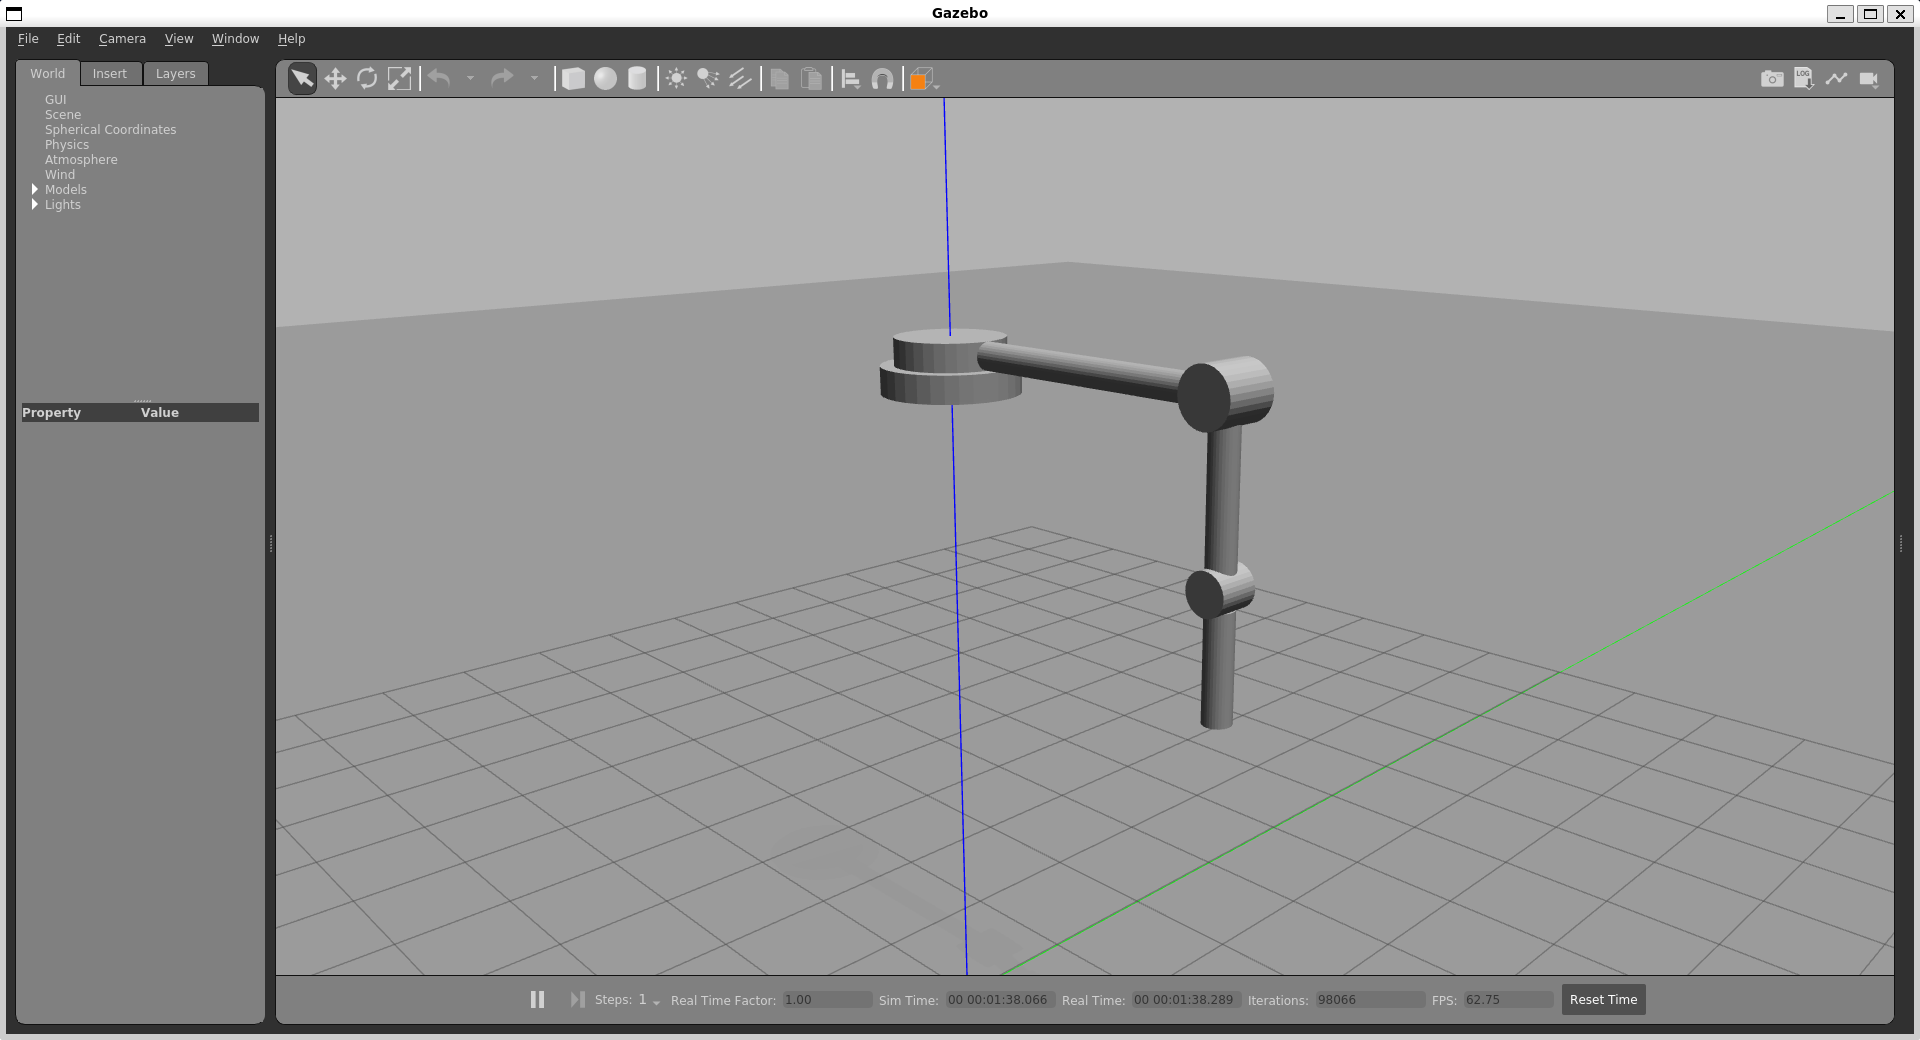
\includegraphics[width=\linewidth]{figures/robotic-arm-gazebo}
        \caption{Gazebo 界面}
    \end{subfigure}
    \hfill
    \begin{subfigure}{0.45\linewidth}
        \centering
        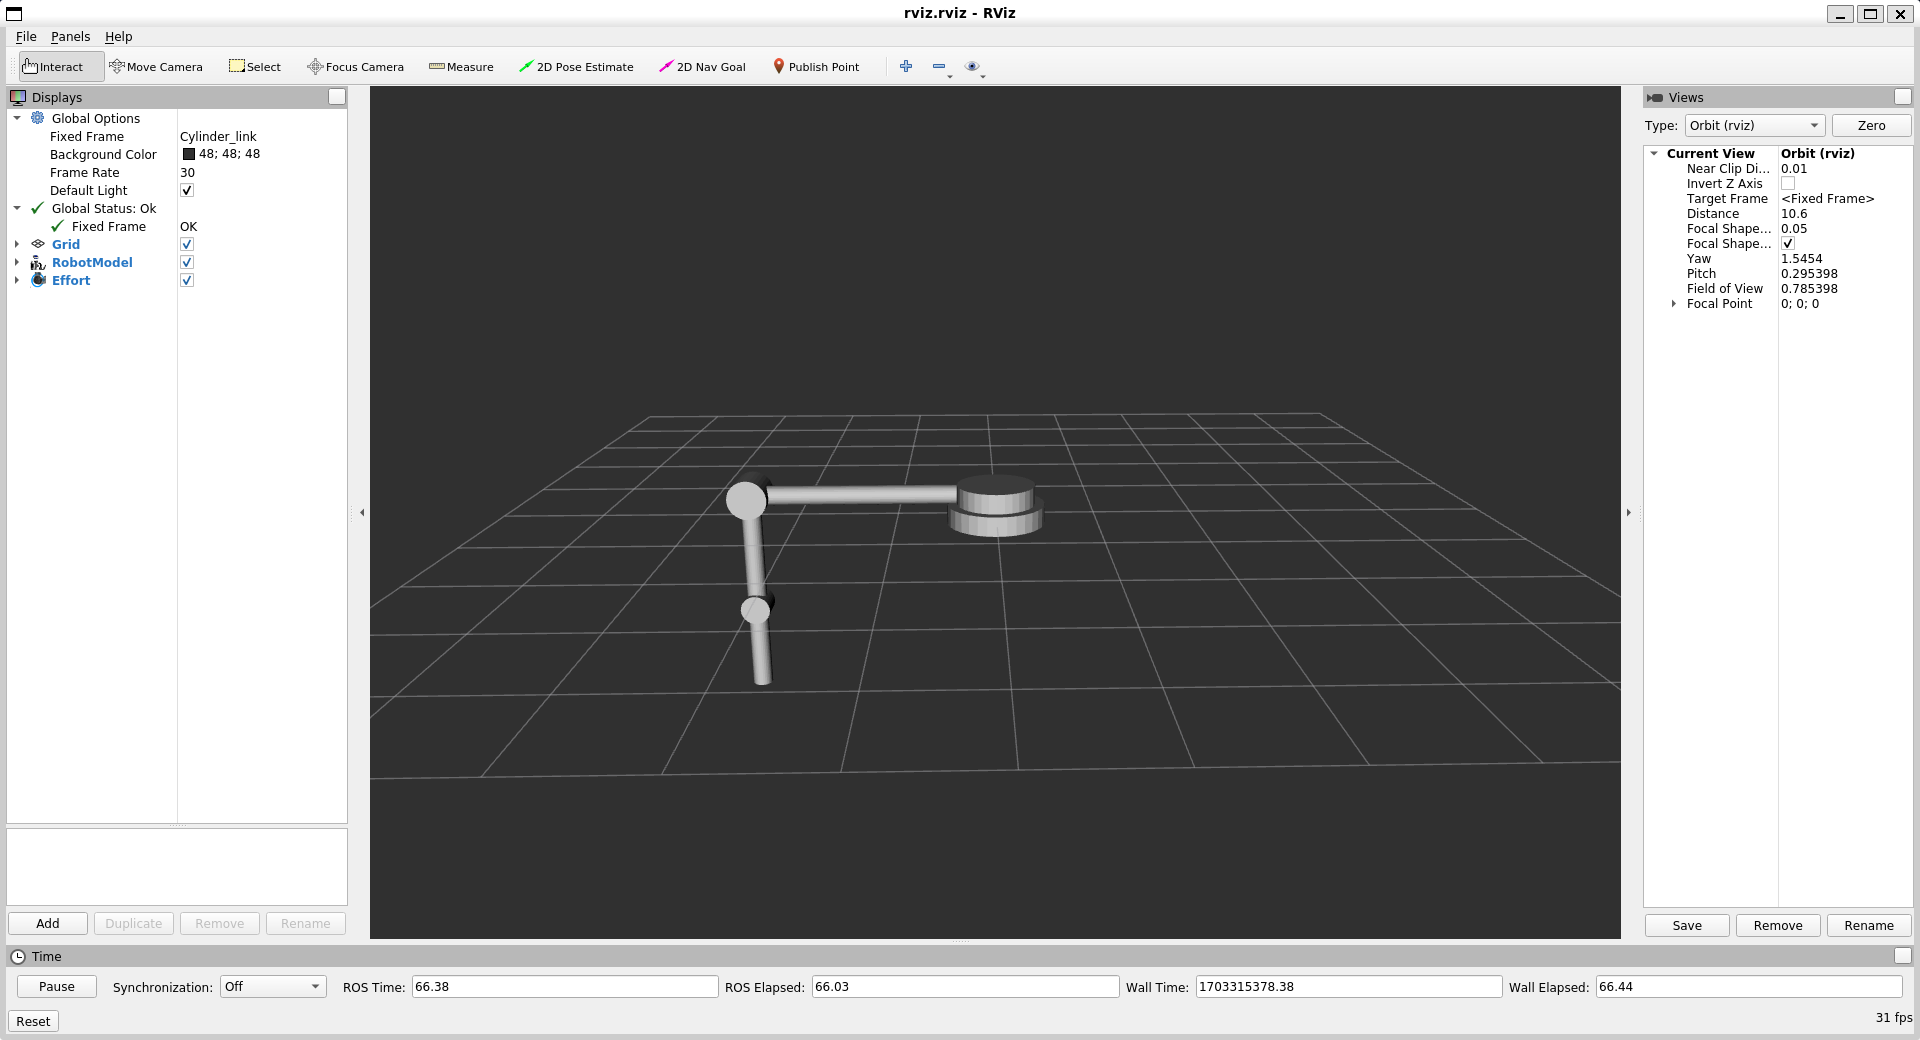
\includegraphics[width=\linewidth]{figures/robotic-arm-rviz}
        \caption{ROS RViz 界面}
    \end{subfigure}
    \hfill
    \caption{仿真使用的模型}
    \label{fig:model}
\end{figure}

我们使用简单的PID控制器对机械臂的前三个转动关节的角度$\theta_{1,2,3}$进行控制。
该控制器由 ROS 中的软件包 \emph{ros\_control} 实现。
通过将控制器参数载入 ROS 参数服务器,在 Gazebo 中加载控制器插件 \emph{gazebo\_ros\_control},在URDF文件中指定传动信息等操作,即可实现机械臂的控制仿真。

我们为每一个关节分配了根据位置控制扭矩的PID控制器,并根据仿真的结果调整参数。
以关节二为例,仿真结果如图\ref{fig:simulated-result-joint-2}所示。

\begin{figure}[ht]
    \centering
    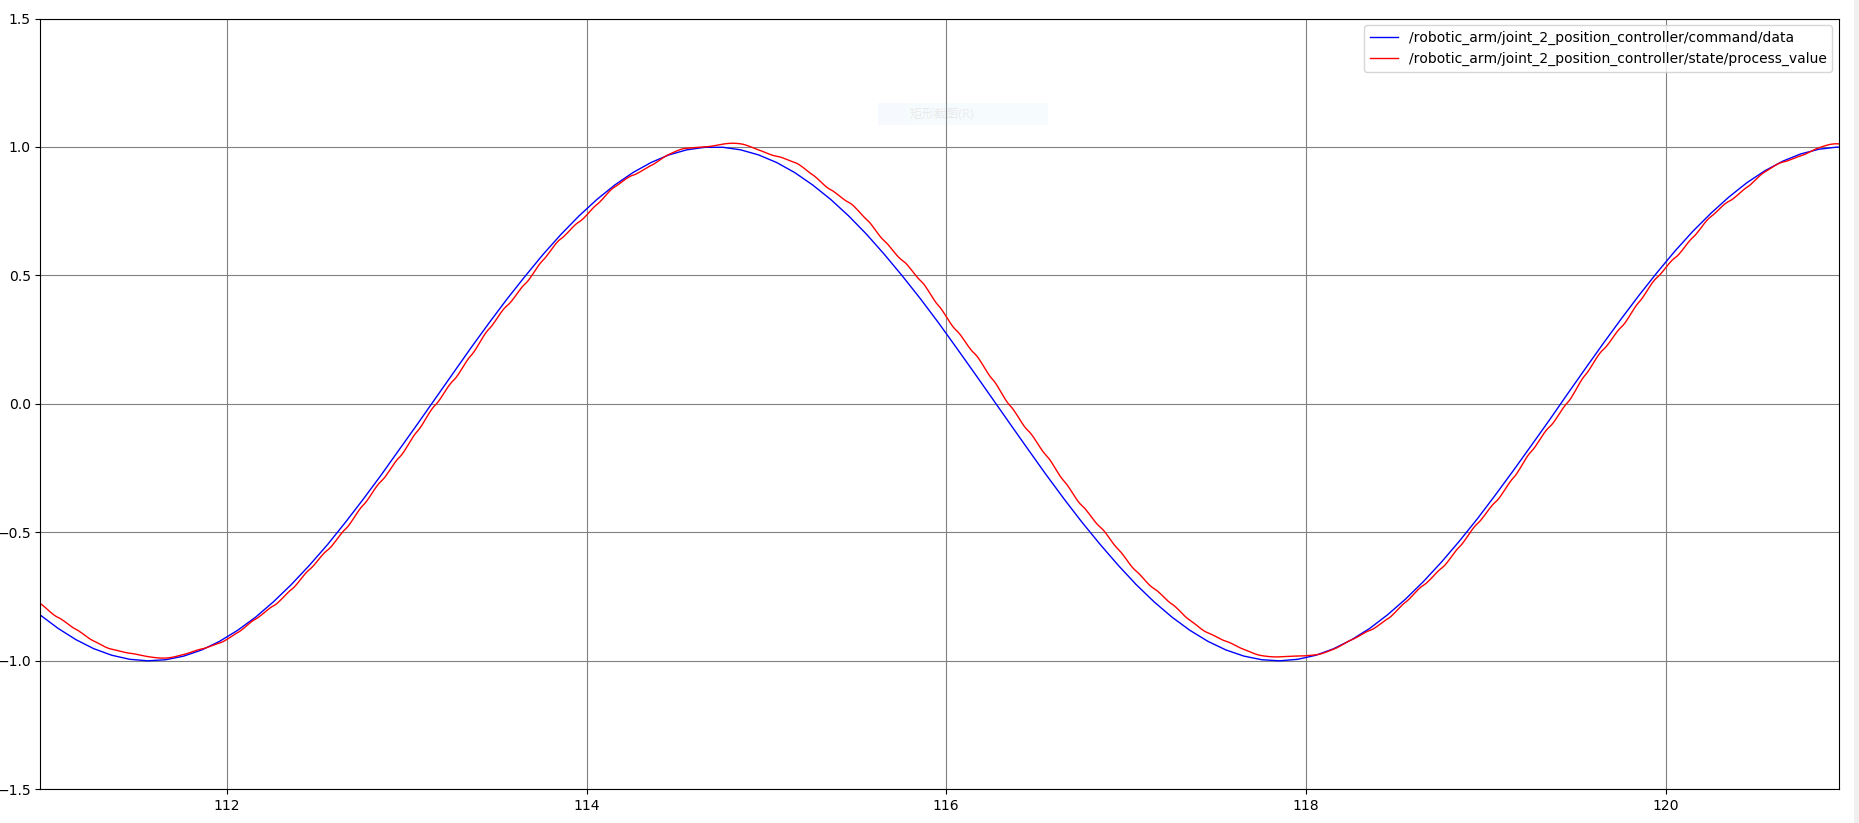
\includegraphics[width=0.8\linewidth]{figures/result-joint-2}
    \caption[关节二仿真结果]{关节二仿真结果(蓝色为指令,红色为关节角度)}
    \label{fig:simulated-result-joint-2}
\end{figure}

仿真中使用的参数为
\[
    \begin{aligned}
        K_p = & \begin{bmatrix}
            1000 & 0 & 0 \\
            0 & 600 & 0 \\
            0 & 0 & 100 \\
        \end{bmatrix} \\
        K_i = & 0.01 \mathbf I \\
        K_d = & 10 \mathbf I
    \end{aligned}
\]

\end{document}
